%----------------------------------------------------------------------------------------
%	CHAPTER 3 // Pupil Eye Tracking Algrithm
%----------------------------------------------------------------------------------------
\chapterimage{Pupil_Chapter_photo4.jpg}
\chapter{Pupil Eye Tracking Algorithm}
As proposed in the previous chapters that we rely on Starburst \cite{starburst} Algorithm to get the center of the pupil. But we found that Starburst is not robust and accurate, so we will use Pupil Algorithm to enhance eye-tracking module. Through this chapter we will go through the details of our eye-tracking module by using Pupil Algorithm.

\section{Pupil}\index{Pupil}
In the second version of our eye-tracking module we went for implementing the Pupil Algorithm \cite{pupil}. Pupil eye-tracking algorithm is an accessible, affordable and extensible tool for pervasive eye tracking research. This chapter we will explain the design motivation of the algorithm, provide an in depth technical description of algorithm. We will use a wearable mobile eye tracking headset with one 
scene camera and one infra-red (IR) spectrum eye camera for dark pupil detection. Both cameras connect to a laptop, desktop, or mobile computer platform via high speed USB 2.0. The camera video streams are read for real-time pupil detection, gaze mapping and recording.  


\section{System Design Objectives}\index{Pupil}
	Pupil leverages the rapid development cycle and scaling effects of consumer electronics, USB cameras and consumer computing hardware, instead of using custom cameras and computing solutions. \bigskip

Pupil algorithm is open source and strives to build and support a community of eye tracking researchers and developers.\cite{pupil}

\section{Cameras} \index{Cameras}
The scene camera mount and eye camera mount interface geometries are open source. By releasing the mount geometry we automatically document the interface, allowing users to develop their own mounts for cameras of their choice. \bigskip \cite{pupil}

Pupil uses USB interface digital cameras that comply with the UVC (USB Video Class) standard. The Pupil headset can be used with other software that supports the UVC interface. Pupil can be easily extended to use two eye cameras for binocular set-ups and more scene cameras as desired. 

\subsection{Eye Camera} \index{Eye Camera}
We use a small and lightweight eye camera to reduce the amount of visual obstruction for the user and keep the headset lightweight. The eye camera can capture at a maximum resolution of 800x600 pixels at 30 Hz. Using an IR mirror ("hot mirror") was considered as  strategy to further reduce visual obstruction.

\bigskip
 Pupil uses the "dark pupil" detection method. This Requires the eye camera to capture video within a specific range of the IR spectrum. \cite{pupil}

 
 \subsection{Scene Camera} \index{Eye Camera}
  The scene camera is mounted above the user’s eye aligning the scene camera optics with the user’s eye along a sagittal plane. The scene camera faces outwards to capture a video stream of a portion of the users FOV at 30Hz. The scene camera lens has a 90 degree diagonal FOV. The scene camera is not only high resolution (max resolution 1920x1080 pixels), but also uses a high quality image sensor. This is very
advantageous for further computer vision and related tasks
performed in software. \cite{pupil}


\section{Computing Device} \index{Computing Device}
The Pupil eye tracking algorithm works in conjunction with standard multi-purpose computers: laptop, desktop, or tablet. Designing for user supplied recording and processing hardware introduces a source for compatibility issues and requires more set-up effort for both users and developers. However, enabling the user to pair the headset with their own computing platform makes Pupil a multi-purpose eye tracking and analysis tool. Pupil is deployable for lightweight mobile use as well as more specialized applications like: streaming over networks, geotagging, multi-user synchronization; and computationally intensive applications like real time 3D reconstruction and localization. \cite{pupil}

\section{Pupil Detection Algorithm} \index{Pupil Detection Algorithm}
The pupil detection algorithm locates the dark pupil in the IR illuminated eye camera image. The algorithm does not depend on the corneal reflection, and works with users who wear contact lenses and eyeglasses. \bigskip

The pupil detection algorithm is under constant improvement based on feedback collected through user submitted eye camera videos. Here we provide a description of default pupil detection algorithm.
\bigskip \cite{pupil}

\subsection{overview} \index{Pupil Detection Algorithm}
The eye camera image is converted to gray-scale. The initial region estimation of the pupil is found via the strongest response for a center-surround feature as proposed by Swirski et al. \cite{swirski} within the image. \newline  

Detect edges using Canny \cite{canny} to find contours in eye image. Filter edges based on neighbouring pixel intensity. Look for darker areas (blue region). Dark is specified using a user set offset of the lowest spike in the histogram of pixel intensities in the eye image. \\*

Filter remaining edges to exclude those stemming from spectral reflections. Remaining edges are extracted into into contours using connected components \cite{suzuki}. Contours are filtered and split into sub-contours based on criteria of curvature continuity. \\*

Candidate pupil ellipses are formed using ellipse fitting \cite{fitzgibbon96} onto a subset of the contours looking for good fits in a least square sense, major radii within a user defined range, and a few additional criteria. \\* 

The results are evaluated based on the ellipse fit of the supporting edges and the ratio of supporting edge length and ellipse circumference (using Ramanujans second approximation \cite{hardy1962collected} ). We call this ratio "confidence". If the best results confidence is above a threshold the algorithm reports this candidate ellipse as the ellipse defining the contour of the pupil. Otherwise the algorithm reports that no pupil was found.\\* 

\begin{figure*}[]
\begin{dBox}
\centering
  \mbox{
	    \subfigure[Algorithm Overview]{
            \label{fig:overview}
            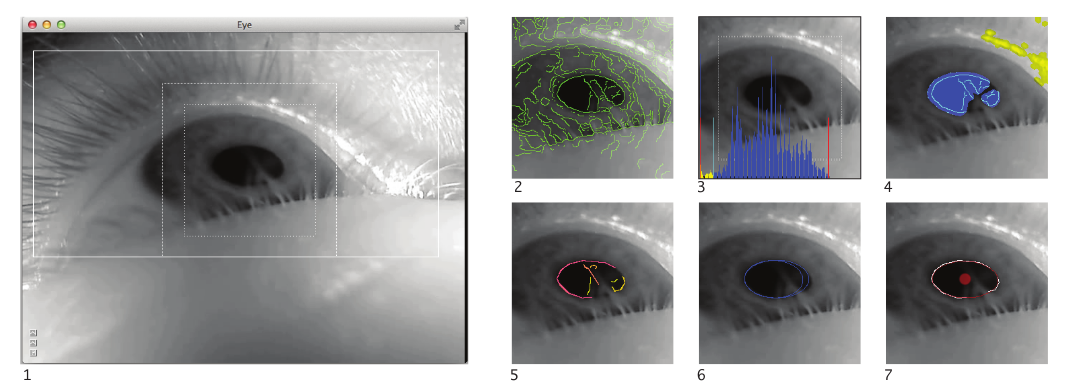
\includegraphics[width=1.0\textwidth]{./Pictures/pupil/Visulaization_of_Pupil_algo.png}
        }
   }
   \caption{Vizualization of pupil detection algorithm. 1) Eye image converted to gray scale, user region of interest (white stroke rectangle), and initial estimation of pupil region (white square and dashed line square.) 2) Canny edge detection (green lines). 3) Define "dark" region as offset from lowest spike in histogram within eye image. 4) Filter edges to exclude spectral reflections(yellow) and not inside "dark" areas (blue). 5) Remaining edges extracted into contours using connected components and split into sub-contours based on curvature criteria (multi colored lines). 6) Candidate pupil ellipses (blue) are formed using ellipse fitting. 7) Final Ellipse fit found through an augmented combinatorial search( finally ellipse with center in red)-supporting edge pixels drawn in white. \cite{pupil}
 \label{fig:Pupil_Performance} }   
\end{dBox}   
\end{figure*}


\begin{figure*}[]
\begin{dBox}
\centering
  \mbox{
	      \subfigure[Comparison]{
            \label{fig:Comparison}
            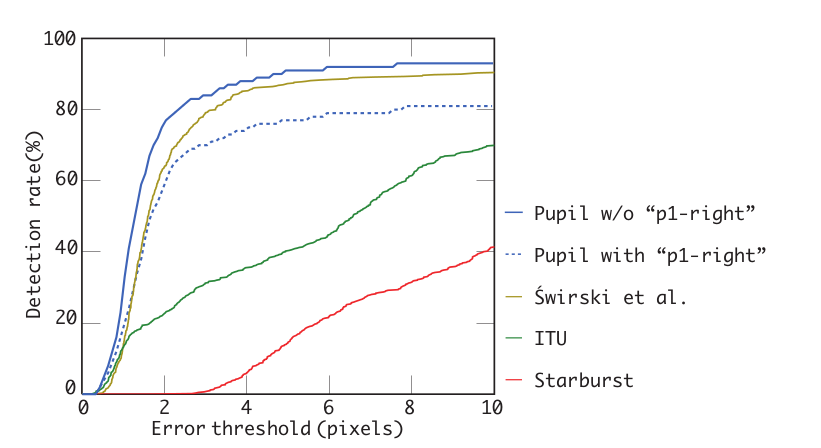
\includegraphics[width=.80\textwidth]{./Pictures/pupil/comparison.png}
        }
   }
   \caption{Comparison of pupil detection rate for Pupil’s algorithm, the stock algorithm proposed by Swirski et al., the ITU gaze tracker and Starburst.\cite{pupil}
 \label{fig:Pupil_Performance} }   
\end{dBox}   
\end{figure*}

Figure \ref{fig:Pupil_Performance} shows a performance comparison between Pupil’s pupil detection algorithm, the stock algorithm proposed by Swirski et al., the ITU gaze tracker and Starburst on the benchmark dataset by Swirski et al. \cite{swirski}. As error measure we used the Hausdorff distance between the detected and hand-labeled pupil ellipses \cite{swirski}. We additionally conducted a test excluding the dataset p1-right, that contains eye images recorded at the most extreme angles.
As can be seen from the Figure, Pupil without p1-right compares favourably to all other approaches. With an error threshold of 2 pixels Pupil achieves a detection rate of 80\%; at 5 pixels error detection rate increases to 90\% \cite{pupil}


\begin{figure*}[]
\begin{dBox}
\centering
  \mbox{
	      \subfigure[Initial Estimation of Pupil Region]{
            \label{fig:Pupil Region}
            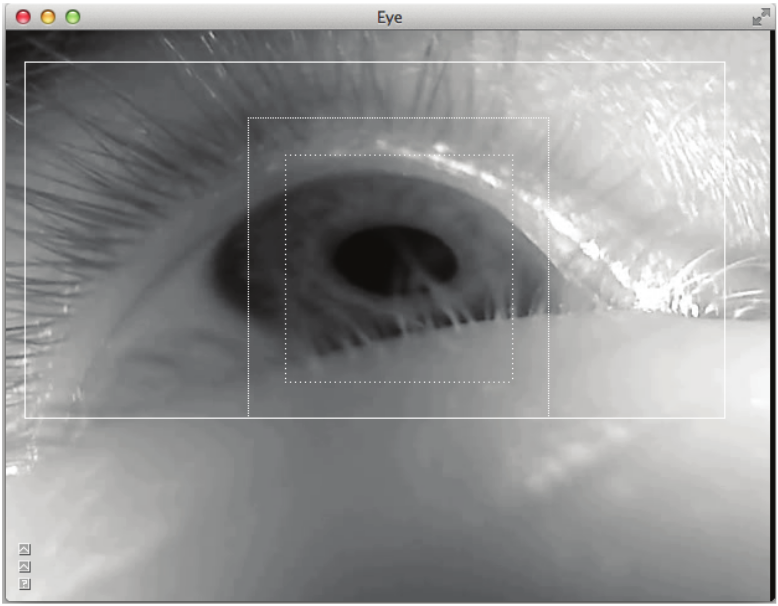
\includegraphics[width=.80\textwidth]{./Pictures/pupil/initial_estimation_of_pupil.png}
        }
   }
   \caption{ User region of interest (white stroke rectangle), and initial estimation of pupil region (white square and dashed line square.)\cite{pupil}
 \label{fig:Pupil Region} }   
\end{dBox}   
\end{figure*}


\begin{figure*}[]
\begin{dBox}
\centering
  \mbox{
	      \subfigure[Estimation of Pupil Region]{
            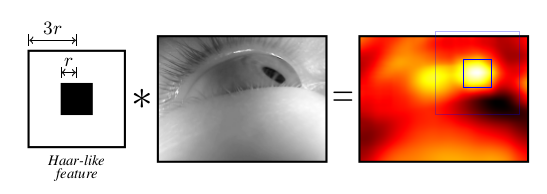
\includegraphics[width=.80\textwidth]{./Pictures/pupil/estimation_pupil_region.png}
        }
   }
   \caption{ To find the approximate pupil region, the eye image is convolved with a Haar-like centre surround feature of radius r. The pupil region is centred on the location of the maximal response over all pixels and radii. \cite{pupil}
 \label{fig:EstimationPupilFig} }   
\end{dBox}   
\end{figure*}


\begin{figure*}[]
\begin{dBox}
\centering
  \mbox{
	      \subfigure[]{
            \label{fig:IntegralImage}
            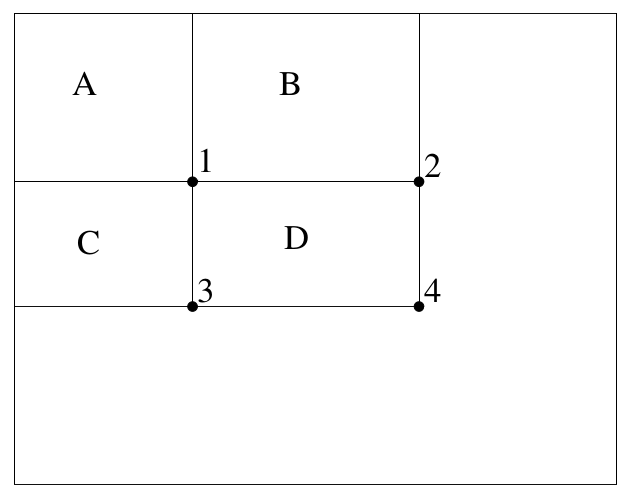
\includegraphics[width=.40\textwidth]{./Pictures/pupil/integral_image.png}
        }
   }
   \caption{ To find the approximate pupil region, the eye image is convolved with a Haar-like centre surround feature of radius r. The pupil region is centred on the location of the maximal response over all pixels and radii. \cite{ViolaAndJones2001}
 \label{fig:IntegralFig} }   
\end{dBox}   
\end{figure*}


\subsection{Integral Image} \index{ Pupil Detection Algorithm }
Rectangle features can be computed very rapidly using an intermediate representation for the image which we call the integral image. The integral image at location $x, y$ contains the sum of the pixels above and to the left of $x, y$, inclusive: \\
\begin{center}
$ii(x,y)=\sum\limits_{x'<=x,y'<= y}i(x', y')$,
\end{center}
where $ii(x,y)$ is the integral image and $i(x,y)$ is the original image. Using the following pair of recurrences:
\begin{center}
	\begin{equation}
	$s(x,y) = s(x,y-1)+ i(x,y)$
	\end{equation}

	\begin{equation}
	$ii(x,y) = ii(x-1,y)+ s(x,y)$
	\end{equation}

\end{center}
(where $ s(x,y) $is the cumulative row sum, $s(x, -1) = 0$, and $ii(-1, y) == 0$) the integral image can be computed in one pass over the original image. \\
Using the integral image any rectangular sum can be computed in four array references figure \ref{fig:IntegralFig}. Clearly the difference between two rectangular sums can be computed in eight references. Since the two-rectangle features defined above involve adjacent rectangular sums they can be computed in six array references, eight in the case of the three-rectangle features, and nine for four-rectangle features.\cite{ViolaAndJones2001}

\begin{figure*}[]
\begin{dBox}
\centering
  \mbox{
	      \subfigure[Original Eye Image]{
	            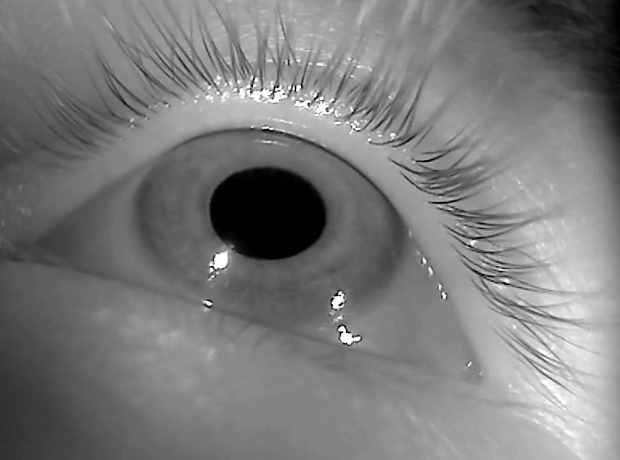
\includegraphics[width=.45\textwidth]{./Pictures/pupil/0-eye.png}
        }
	      \subfigure[Region of interest(ROI) after Running Initial Estimation Of Pupil Module]{
	      		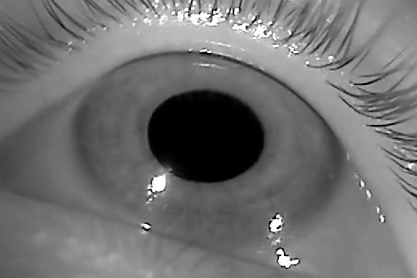
\includegraphics[width=.50\textwidth]{./Pictures/pupil/ROI.png}
        }
   }
   
   \caption{Input \& Output of Initial Estimation of Pupil Module. \label{fig:Initial_Estimation_Of_Pupil} }   
\end{dBox}   
\end{figure*}

\subsection{Initial Estimation Of Pupil} \index{Pupil Detection Algorithm}
Our initial region estimation assumes that the pupil region, either the dark pupil itself or the combination of pupil and iris, can roughly be described as a “ dark blob surrounded by a light background ”, and is the strongest such feature in the image. To find the pupil, we use a Haar-like feature detector, similar to the features used in cascade classifiers \cite{ViolaAndJones2001}. \bigskip

The core idea of the feature detector can be explained in terms of convolution. To find possible pupil regions, we convolve the image with a Haar-like centre-surround feature of a given radius figure \ref{fig:EstimationPupilFig} . We repeat this for a set of possible radii, between a user specified minimum and maximum, and find the strongest response over the 3D space of (x, y) and radii. The (x, y) location of this strongest response is assumed to be the centre of the pupil region, with the size of the region determined by the corresponding radius. \bigskip

Although such a convolution is a slow operation if performed naively, we optimise this by first calculating the integral image \cite{ViolaAndJones2001}. Using this integral image, we can find the response of a pixel to a Haar-like feature in constant time, only needing to sample 8 pixel values, one for each corner of the two squares, thereby making this step linear in the number of pixels and possible radii. \\
Input and Output of this module is shown in Figure \ref{fig:Initial_Estimation_Of_Pupil}

\begin{figure*}[]
\begin{dBox}
\centering
  \mbox{
	      \subfigure[Eye Image after Computing Histogram]{
	            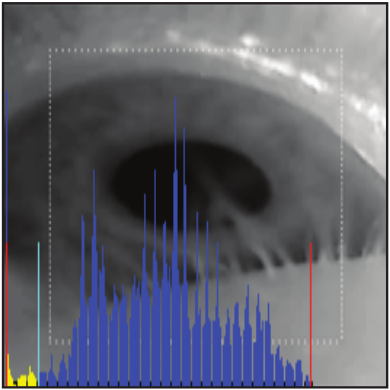
\includegraphics[width=.40\textwidth]{./Pictures/pupil/histogramOnDarkRegion.png}
        }
   }
   \caption{After Computing Histogram to get Spikes. \cite{pupil}
   \label{fig:HistogramOnEyeImage} }   
\end{dBox}   
\end{figure*}

\begin{figure*}[]
\begin{dBox}
\centering
  \mbox{
	    \subfigure[Eye image after applying Closing operation on Eye image.]{
	          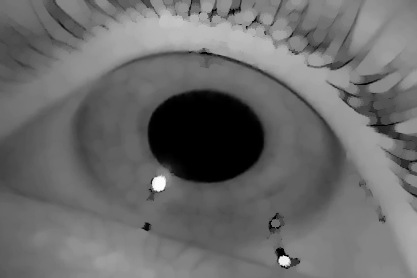
\includegraphics[width=.60\textwidth]{./Pictures/pupil/dark_region_img.png}
        }
        	\subfigure[Dark region is indicated by the Blue Region]{
        		  \label{fig:SpectralReflection} 
	          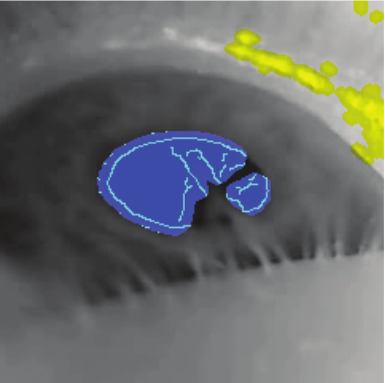
\includegraphics[width=.40\textwidth]{./Pictures/pupil/DarkRegion.png}
        }

   }
   \caption{After Applying Morphological operations(Closing operations).\cite{pupil} 
   \label{fig:DarkImageInBlue} }   
\end{dBox}   
\end{figure*}


\begin{figure*}[]
\begin{dBox}
\centering
  \mbox{
	    \subfigure[Eye image after applying Closing operation on Eye image.]{
	          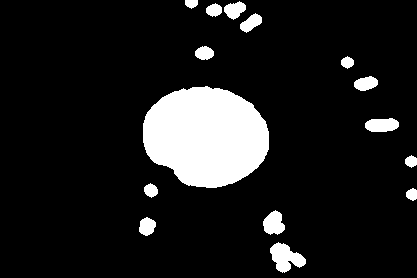
\includegraphics[width=.30\textwidth]{./Pictures/pupil/dark_region_binary_img.png}
        }
   }
   \caption{Final Result of Getting Dark Region Module. 
   \label{fig:DarkImageInBinary} }   
\end{dBox}   
\end{figure*}


\subsection{Getting Dark Region(Pupil Region)} \index{Pupil Detection Algorithm}
Here we want to extract the region which include the pupil by getting the most dark region in eye image. And then we filter the eye image by applying some Morphological operations like Dilation and Erosion to remove the noise to get a pure dark region. \bigskip

At first we should get the histogram of the gray image of Region Of Interest (ROI) which we get from Initial Estimation Of Pupil Module. Then we should deduce spikes from histograms. After getting the lowest and highest spikes in histogram we can get the binary image of ROI by using lowest spike +  user offset(usually we set offset by 11) as threshold as shown in figure \ref{fig:HistogramOnEyeImage}. \bigskip

Then, we should do some Morphological operation on binary image. to filter the image from any noise and make contours more clearer, so we apply Erosion at first and then Dilation(Closing Operation) as shown in Figure \ref{fig:DarkImageInBlue}. \bigskip

Finally we get the ROI as a binary image include only the Dark Region which represents Pupil as shown in Figure \ref{fig:DarkImageInBinary}.


\begin{figure*}[]
\begin{dBox}
\centering
  \mbox{
	    \subfigure[Edges of eye image after Excluding Spectral Reflections]{
	          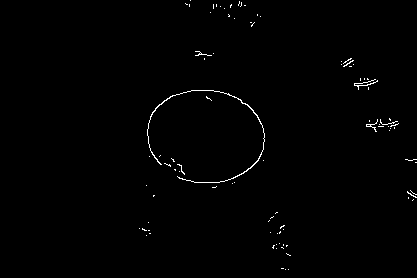
\includegraphics[width=.50\textwidth]{./Pictures/pupil/edges_after_Removing_Spectral_Refl.png}
        }
   }
   \caption{Final Result of Excluding Spectral Reflection module.
   \label{fig:Edges} }   
\end{dBox}   
\end{figure*}

\subsection{Excluding Spectral Reflection} \index{Pupil Detection Algorithm}
	We need to filter all the edges which result from Canny edge detector, by excluding the spectral reflection which appears as yellow lines in figure \ref{fig:SpectralReflection} that is out of the dark region. So, we need to remove edges in areas which are not dark enough and where the glints is (Spectral Reflection from IR leds).\bigskip
		
	We get minimum edges from comparing edges image which result from Canny edge detector with the Spec Mask (Mask that we get from the in range thresholding with highest spike and 255) and then we reduce the number of edges by comparing the edges image with binary Mask(Mask which we get from in range thresholding with lowest spike with 255).\bigskip

	At the end we remove the Spectral reflection and the binary eye image is filtered from any noise as shown in Figure \ref{fig:Edges}. 
	 


\begin{figure*}[]
\begin{dBox}
\centering
  \mbox{
	    \subfigure[Multi coloured lines represent different contours ]{
	          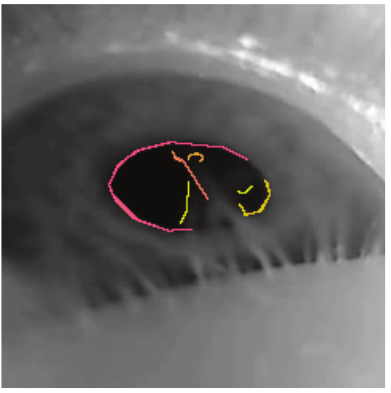
\includegraphics[width=.30\textwidth]{./Pictures/pupil/contours.png}
        }
   }
   \caption{Final Result of Extracting Contour module. \cite{pupil}
   \label{fig:Contours} }   
\end{dBox}   
\end{figure*}


\subsection{Extracting Contours} \index{Pupil Detection Algorithm}
	After getting the minimum edges we can extract Contours by using connected components, and then split the contours into sub-contours based on curvature continuity criteria as shown in Figure \ref{fig:Contours}. \cite{suzuki} \bigskip
	We have used OpenCV findCountours method to get all the contours from edges and then we get the approximate Poly-lines that each contour forms. So that, we can use each poly-line to get the angle between each subsequent 2 points to make sure that this contour is a good contour and also it helps to split contours into sub-contours based on angles between two subsequent points.  


\begin{figure*}[]
\begin{dBox}
\centering
  \mbox{
	    \subfigure[Final ellipse with center in red and supporting edge pixels are drawn in white.]{
	          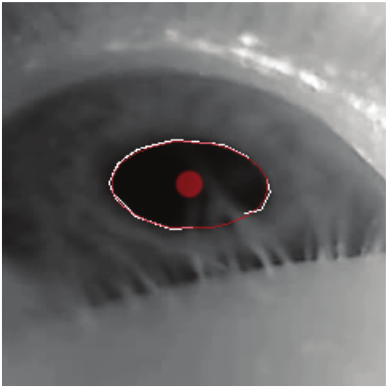
\includegraphics[width=.30\textwidth]{./Pictures/pupil/final_ellipse.png}
        }
   }
   \caption{Final Result of Ellipse Fitting module.\cite{pupil}
   \label{fig:EllipseFit} }   
\end{dBox}   
\end{figure*}


\subsection{Ellipse Fitting} \index{Pupil Detection Algorithm}
	Finally we should estimate the best ellipse that surrounds the Pupil by fitting an ellipse found through an augmented combinatorial search. \cite{fitzgibbon96} \bigskip
	
	Candidate pupil ellipses are formed using ellipse fitting onto a subset of the contours looking for good fits in a least square sense, major radii within a user defined range and a few additional criteria. An augmented combinatorial search looks for contours that can be added as support to the candidate ellipses. The results are evaluated based on the ellipse fit of the supporting edges and the ratio of supporting edge length and ellipse circumference. We call this ratio “ confidence ”. If the best results confidence is above a threshold the algorithm reports this candidate ellipse as the ellipse defining the contour of the pupil as shown in Figure \ref{fig:EllipseFit}. Otherwise the algorithm reports that no pupil was found. \bigskip \cite{pupil}

	
\section{Performance Evaluation} \index{Performance Evaluation}
	We have used Data Set of Computer Laboratory, University of Cambridge, United Kingdom which is used at Robust real-time pupil tracking in highly off-axis images to test performance. \cite{swirski} \\
	These Data Set contains video frames as individual images, and a text file describing the pupil ellipse in selected frames. The format of each line in text file is $<$frame \#$>$ $| <x> <y> <a> <b> < \theta >$, such that $ x , y$ represents the pupil center in frame\# , $ a, b$ represents the ellipse major radius and minor radius  values and $\theta$ represents angle between the major axis and the x-axis in radians. Total number of frames is 940 frame. \\
	Finally after Testing our implementation on this Data Set, we have make a comparison between our results and the original pupil center location. You Can see the Error graph in Figure \ref{fig:ErrorGraph}.\cite{pupil}
		

\begin{figure*}[]
\begin{dBox}
\centering
  \mbox{
	    \subfigure[]{
	          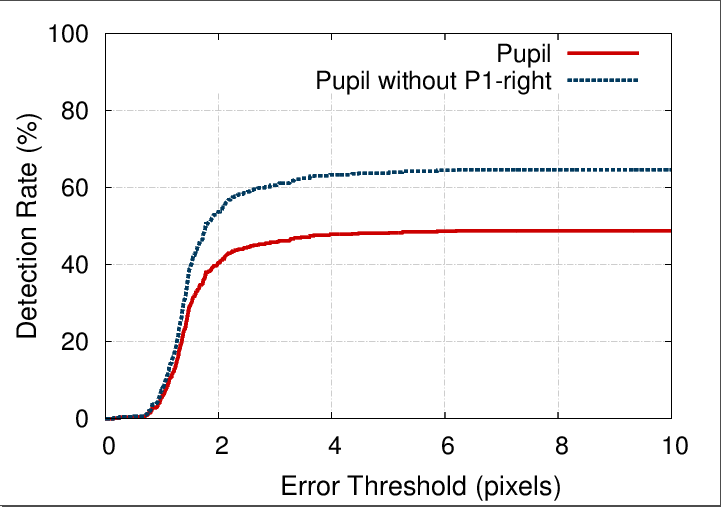
\includegraphics[width=.80\textwidth]{./Pictures/pupil/error_graph.png}
        }
   }
   \caption{Error graph for Pupil algorithm performance test.
   \label{fig:ErrorGraph} }   
\end{dBox}   
\end{figure*}
